%% статьи в формате LaTeX для сборника статей "Системное         **
%% **  программирование".                                                   **
%% **  СПбГУ, мат.-мех. факультет, НИИ ИТ, 2005 г.                          **
%% **  Текст собирается с помощью программы latex                           **
%% **                                                                       **
%% ***************************************************************************

\documentclass[a5paper]{article}
\usepackage[a5paper, top=17mm, bottom=17mm, left=17mm, right=17mm]{geometry}
\usepackage[T2A]{fontenc} 
\usepackage[utf8]{inputenc}
\usepackage[english,russian]{babel}
\usepackage{graphicx}
\usepackage{indentfirst}
\usepackage{hyperref}
\usepackage{textcomp}


\sloppy
\pagestyle{empty}

%% ***************************************************************************
%% **                                                                       **
%% **  Место для названия статьи                                            **
%% **                                                                       **
%% ***************************************************************************
\title{Generalized LL parsing for context-free constrained path search problem}

%% ***************************************************************************
%% **                                                                       **
%% **  Место для авторов, их email-адресов и названий институтов            **
%% **                                                                       **
%% ***************************************************************************
\author{Semyon Grigorev\\
rsdpisuy@gmail.com\\
Saint-Petersburg State University, Russia}
%198504, Университетский проспект, 28, Старый Петергоф,\\
%Санкт-Петербург, Россия}
%\date{}
\begin{document}

\maketitle
%\thispagestyle{empty}

%% ***************************************************************************
%% **                                                                       **
%% ** Аннотация                                                             **
%% **                                                                       **
%% ***************************************************************************
%\begin{quote}

%\renewcommand{\thefootnote}{}

%% ***************************************************************************
%% **                                                                       **
%% ** Авторские права                                                       **
%% **                                                                       **
%% ***************************************************************************
%\setcounter{footnote}{0}
%\end{quote}

%% ***************************************************************************
%% **                                                                       **
%% ** Текст статьи                                                          **
%% **                                                                       **
%% ***************************************************************************
\section{Introduction}

In ~\cite{DirOfBigGraphAnalysis} some problems on formal languages path problems are formulatred. We want to propose an idea of context-free languages constrained path problem solution. 
It is based on generalized LL (GLL)~\cite{GLL} parsing algorithm which allow to process arbitrary context-free grammars.

\section{Generalised LL parsing}


\section{Graph processing with generalised LL}

We can specify path constraint as context-free grammar.

\begin{verbatim}
s: A s B | eps
\end{verbatim}



\section{Generalized LL for path searching}

Full index --- for dynamic graphs. It is necessary only recalculate ... This operation is native for basic algorithm.

\section{Discussion}



%\begin{figure}
%    \begin{center}
%        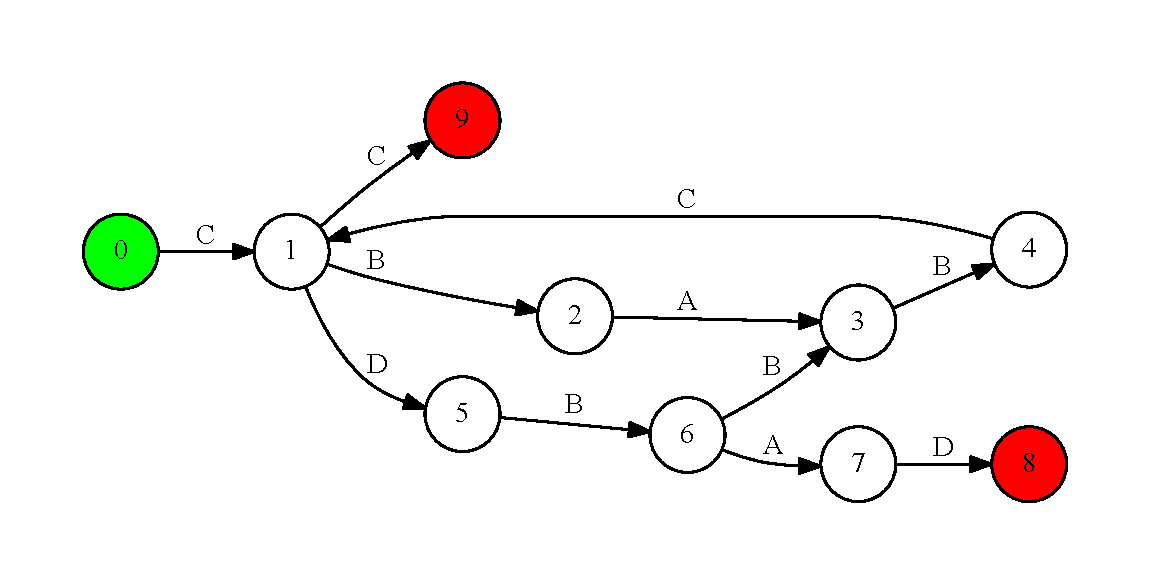
\includegraphics[width=11cm]{input.pdf}
%        \caption{Входной граф}
%        \label{pic1}        
%    \end{center}
%\end{figure}
%


%% ***************************************************************************
%% **                                                                       **
%% ** Список литературы                                                     **
%% **                                                                       **
%% ***************************************************************************
\begin{thebibliography}{99}
  
\bibitem{DirOfBigGraphAnalysis}
Miller, J. A., Ramaswamy, L., Kochut, K. J., \& Fard, A. (2015, June). Research Directions for Big Data Graph Analytics. In 2015 IEEE International Congress on Big Data (pp. 785--794). IEEE.

\bibitem{GLL}
Scott, E., \& Johnstone, A. (2010). GLL parsing. Electronic Notes in Theoretical Computer Science, 253(7), 177--189.

\end{thebibliography}

\end{document}
